% This is samplepaper.tex, a sample chapter demonstrating the
% LLNCS macro package for Springer Computer Science proceedings;
% Version 2.20 of 2017/10/04
%
\documentclass[runningheads]{llncs}
%
\usepackage{graphicx}
\usepackage{algorithm} % for algorithms
\usepackage{algpseudocode}
\usepackage{booktabs} % For formal tables
\usepackage{amsthm} % For claims
\usepackage{bbm} % indicator function

\usepackage{cite}

% \usepackage{subfig}
\usepackage{subcaption}

% listings
\usepackage{xcolor,listings}
\usepackage{textcomp}
\lstset{upquote=true}

% plots
\usepackage{pgfplots}

% table
\usepackage[flushleft]{threeparttable} % http://ctan.org/pkg/threeparttable
\usepackage{booktabs,caption}

\theoremstyle{remark}

% Used for displaying a sample figure. If possible, figure files should
% be included in EPS format.
%
% If you use the hyperref package, please uncomment the following line
% to display URLs in blue roman font according to Springer's eBook style:
% \renewcommand\UrlFont{\color{blue}\rmfamily}

\begin{document}
%
\title{Towards Adaptive SQL Query Optimization in Distributed Stream Processing}
%
\titlerunning{Distributed Streaming SQL Optimization}
% If the paper title is too long for the running head, you can set
% an abbreviated paper title here
%
\author{Darya Sharkova\inst{1} \and
Alexander Chernokoz\inst{2} \and
Artem Trofimov\inst{3} \and
Nikita Sokolov\inst{3} \and
Ekaterina Gorshkova\inst{4} \and
Igor Kuralenok\inst{3}\and
Boris Novikov\inst{1}}
%
\authorrunning{D. Sharkova, A. Chernokoz et al.}
% % First names are abbreviated in the running head.
% % If there are more than two authors, 'et al.' is used.
% %
\institute{HSE University, Saint Petersburg, Russia \\ % \\ 
\and
IFMO University, Saint Petersburg, Russia
%\\ 
\and
Yandex, Saint Petersburg, Russia\\
%\email{\{trofimov9artem,faucct,ikuralenok\}@gmail.com} 
\and
JResearch Software, Prague, Czech Republic \\ \email{sharkovadarya@gmail.com}, \email{chernokoz@hotmail.com},
\email{\{trofimov9artem,faucct\}@gmail.com},  \email{cathy@jresearch.org}, \email{ikuralenok@gmail.com},
\email{borisnov@acm.org}
}
%
\maketitle              % typeset the header of the contribution
%
\begin{abstract}
Distributed stream processing is widely adopted for real-time data analysis and management. SQL is becoming a common language for robust streaming analysis due to the introduction of time-varying relations and event time semantics. However, query optimization in state-of-the-art stream processing engines (SPEs) remains limited: runtime adjustments to execution plans are not applied. This fact restricts the optimization capabilities because SPEs lack the statistical data properties before query execution begins. Moreover, streaming queries are often long-lived, and these properties can be changed over time. 

Adaptive optimization, used in databases for queries with insufficient existing data statistics, can fit the streaming scenario. In this work, we explore the main challenges that SPEs face during the adjustment of adaptive optimization: retrieving and predicting statistical data properties, execution graph migration, misfit of SPEs programming interfaces, etc. We demonstrate the feasibility of the proposed approach within an extension of the Nexmark streaming benchmark and outline our further work on this topic.

% \keywords{First keyword  \and Second keyword \and Another keyword.}
\end{abstract}



\section{Introduction}
\label {fs-optimization-introduction}

Modern day data analytics commonly requires online processing of continuously changing data from unbounded streams. A standard way of defining a stream processing pipeline is an execution graph. An alternative would be a declarative approach, which SQL is a popular example of.

For each declarative query, which is translated into a graph upon execution, there can be multiple execution graphs. The best execution graph is selected during \textit{optimization}. In databases, query optimization routinely employs a cost-based approach, which estimates a cost function value for each considered plan and selects the plan (which is a graph with nodes representing query operators) with the minimum cost value. The cost function is typically estimated based on relation cardinality and operator selectivity. Therefore, cost-based optimization requires knowledge of statistical information \cite{Neumann2018optimization}. However, obtaining such knowledge in streaming systems presents certain difficulties.

Efforts to optimize streaming queries execution focus on finding a suitable mapping from a logical graph to a physical graph \cite{grulich2020grizzly, gedik2009code}; such optimizations are local, and in order to perform global optimization, the planner needs to optimize the logical graph as well. The problem of logical level declarative query optimization is currently relevant and presents a challenge.

In this work, we present a detailed analysis of the problem of streaming SQL queries optimization and the challenges in implementing its solution. We also describe preliminary experiments that we have conducted in order to demonstrate feasibility of streaming SQL optimization.  


\section{Problem statement}
\label {sec:fs-optimization-problem-statement}

To illustrate the problem of streaming SQL query optimization, let us consider an example query, written using the NEXMark \cite{tucker2008nexmark} benchmark model simulating an online auction:

    \begin{lstlisting}[
           language=SQL,
           showspaces=false,
           basicstyle=\ttfamily,
           numbers=left,
           numberstyle=\tiny,
           commentstyle=\color{gray},
           caption={The proposed NEXMark-based query}, 
           captionpos=b
        ]
SELECT P.name, B.price, A.itemName 
  FROM Person P 
    INNER JOIN Bid B 
      ON B.bidder = P.id 
    INNER JOIN Auction A 
      ON A.seller = P.id
\end{lstlisting}

This query contains two join operators, so there are at least two ways to execute this query: e.g. first performing the join between \texttt{Person} and \texttt{Auction}, then joining the result with \texttt{Bid}, or vice-versa. Which join order is more optimal depends on the statistical properties of the data, such as the arrival rate for each of the \texttt{Person}, \texttt{Auction}, \texttt{Bidder} streams, and such statistical properties have a tendency to change over time. Therefore, an execution graph that was once optimal might become inefficient after some time.

Various DBMS have employed a technique known as adaptive optimization. This technique utilizes an \textit{adaptivity loop}, during which the system measures and evaluates data characteristics and uses these evaluations to select a new query plan better suited to the current data \cite{deshpande2007adaptive}. A similar technique could be useful in streaming queries optimization. Thereby, in this paper we consider the problem of adaptive optimization of streaming SQL queries in distributed stream processing systems. 

Adaptive database optimization is not applicable to streaming SQL queries as is: in databases, such optimization is applied during the execution of a long-running query, with the queried data remaining the same, while in streaming systems the data is continuously updated, and the same query is executed on each subsequent window; therefore, it would make sense for streaming systems to optimize the execution graph between the windows. This presents certain challenges in implementing logical level streaming query optimization.



\section{Challenges}
\label {sec:fs-optimization-challenges}

\textbf{Fetching and predicting statistics.} Cost-based optimization requires statistical information on data in order to calculate cost function values for each plan. However, upon the start of a streaming query execution no information about the data is available. Therefore, in order to properly apply cost-based optimization to streaming SQL queries, it is necessary to collect data statistics over the course of query execution; it's important to note that this should be implemented without significantly impacting the performance. Moreover, since we possess no definitive knowledge about the arriving data, in order to utilize an optimal plan for the upcoming windows, we need to predict statistics for each next window based on statistics for previous windows.

\textbf{Using statistics for query optimization.} The API of the current state-of-the-art systems typically utilizes a top-down approach to building a graph for query execution: first, a logical graph is created, then it is transformed into a physical graph, which is later used for execution, leaving no opportunity to pass any data from the physical level to the logical level and use it to adapt the graph to the new data and therefore making any runtime adjustments to execution plans impossible. Thus, the streaming systems API should be modified in order to make the passing of statistical information from the physical graph to the query planner possible.

\textbf{Execution graph migration at runtime.} Even if the optimal query execution plan was selected based upon statistics accumulated for previous windows, the new data statistics might be different enough to render the previous plan no longer optimal. In order to adapt to the changes in data, it's necessary to identify the moment in time in which the previous plan is no longer optimal for the current or upcoming data and to migrate the execution to a new graph. The graph migration could be implemented in a manner similar to the parallel track strategy \cite{zhu2004dynamic}, where the new execution graph is deployed alongside the old one, whose execution is terminated once it had finished processing the current window. Determining at which point the graph migration would be beneficial to perform (would cause a gain in performance despite the migration costs) is also a challenge.

\subsection{Fetching and predicting data statistics}
Cost-based optimization requires statistical information on data in order to calculate cost function values for each plan. However, upon starting a streaming query execution, no information about the data, such as its arrival rate, is available. 
Therefore, to properly apply cost-based optimization to streaming SQL queries, it is necessary to collect data statistics for query execution. 
Moreover, since we possess no definitive knowledge about the arriving data, we need to predict statistics for each next window based on statistics for previous windows to utilize an optimal plan for the upcoming windows. To this end, we identify two challenges in using statistics for streaming query optimization:

\begin{itemize}
    \item \textbf{Engineering}:
    Statistical information on stream elements, such as their arrival rate, needs to be collected during execution at runtime without seriously affecting the performance of a distributed SPE. % which can present certain challenges since there is no centralized point at which to collect statistics, so we would need to aggregate it somehow, which can affect the performance of the system itself
    \item \textbf{Research}
We need techniques to predict statistics for upcoming windows based on statistics collected for previous windows.    
We expect that previous window statistics would present a decent baseline. 
However, this assumption requires further investigation. 
\end{itemize}

Popular SPEs and frameworks for defining streaming workflows do not offer any statistics fetching or predicting. 
For example, the Apache Beam framework passes constant values to the query planner instead of any actual data statistics to
 Apache Calcite, a dynamic data management framework that implements its SQL processing functionality.



\subsection{Using statistics for streaming query optimization}
% is it plural. is it APIs??
The API of the current state-of-the-art systems typically utilizes a top-down approach to building a graph for query execution: first a logical graph is created, then it is transformed into a physical graph, which is later used for execution, leaving no opportunity to pass any data from the physical level to the logical level and use it to adapt the graph to the new data and therefore making any runtime adjustments to execution plans impossible. While progress has been made in applying various optimizations to the execution graphs at the physical level (see \cite{grulich2020grizzly} or Google Cloud Dataflow optimizer), there are no significant results in logical level optimization yet, and the logical level allows for more complex optimizations than the physical level. Moreover, in this paper we discuss distributed stream processing engines, which require additional consideration when it comes to query execution. To this end, we identify the following challenges:

\begin{itemize}
    \item \textbf{Technical}: it is necessary to adapt the API of current SPEs to pass statistics collected or predicted during the query execution at the physical level to the query planner at the logical level.
    \item \textbf{Research}: the relational algebra and the planner cost model should be extended with new operators specific to distributed systems. For example, a join operation performed upon a stream with a low arrival rate of new elements would be broadcasted to all the nodes in the system, while a high arrival rate suggests distributing different keys across different nodes. Therefore, a new \textit{distribution} operator should be included into the relational algebra, and the cost model should include the estimate of its cost. The cost model should consider the latency due to communication between nodes as well. Such cost models have been well-researched in distributed databases \cite{kossmann2000thestate} but not in distributed streaming systems.
\end{itemize}


% original notes
% state of the art systems API is top-down approach we create logical graph its transformed into physical and there's no way to pass info from execution to building graph level and we need that to migrate graph in runtime

% had it not been for idea to optimize logical graph and more complicated optimizations we do need to pass that info

% my only citation for dataflow is https://doi.org/10.1145/3328905.3338223 and idk if keynotes count as actual citations!

\subsection{Execution graph migration in runtime}
Streaming data is ever-changing: new data continues to arrive indefinitely, and the statistics for the following window elements might differ significantly from the statistics for previous windows. 

Even if the optimal query execution plan was selected based upon statistics accumulated for previous windows, the new data statistics might be different enough to render the previous plan no longer optimal. Therefore, to adapt to the changes in data, it is necessary to identify the moment in time in which the previous plan is no longer optimal for the current or upcoming data and to migrate the execution to a new graph. 

We identify the following challenges in migrating the execution graph in runtime:
\begin{itemize}
 \item \textbf{Research}: identifying the point in time at which it is feasible and beneficial to perform the graph migration is an open problem. First of all, it is necessary to estimate the costs of graph migration at the current point in time. Secondly, we need to establish what qualifies as substantial enough change in statistics to warrant graph migration. 

 \item \textbf{Engineering}: 
    the mechanics of graph migration, particularly for stateful operations such as joins and aggregations, in runtime have been researched~\cite{zhu2004dynamic}.
 However, most current popular SPEs do not provide such functionality. 
   \end{itemize}
One such strategy is the parallel track strategy described in~\cite{zhu2004dynamic}. 
The second graph can start the query execution and the first one, while the first one stops execution when the current window terminates. So all the subsequent windows are only processed by the new execution graph.



\section {Preliminary experiments}
\label {sec:fs-optimization-experiments}
In this section, we describe the preliminary experiments that we conducted in order to demonstrate how the choice of a query plan affects the performance. We aim to show that a well-timed switch from an execution graph that is no longer optimal for the current data to a more optimal one would improve performance significantly. First, we present the experiment setup and the configuration used; then, we demonstrate our results. 
% мы хотим показать, что своевременное переключение между планами может улучшить перформанс; мы просто показываем, что разные планы дают разный перформанс, и поэтому переключение между ними дало бы улучшение
\subsection{Setup}

For our experiments, we used the same query that was described in Section \ref{sec:fs-optimization-problem-statement} and the Apache Beam implementation of the NEXMark benchmark model. In this implementation, each entity (\texttt{Person}, \texttt{Auction}, or \texttt{Bid}) is represented via a subclass of the \texttt{Event} class. Each event is generated by an unbounded source in accordance to the provided configuration, which includes parameters such as the arrival rate for each event, the $|Person|:|Auction|:|Bid|$ ratio, the time-based window size, etc. 

First, we execute this query using the plan in which \texttt{Auction} and \texttt{Person} are joined first, and the result is joined with \texttt{Bid}; then, we use the plan in which \texttt{Person} and \texttt{Bid} are joined first (see Section  \ref{sec:fs-optimization-problem-statement}). For each run, we use a different $|Person|:|Auction|:|Bid|$ ratio.

To evaluate performance, we measure latency and throughput for each window. For a join result, we consider \textit{latency} to be the difference between the maximum arrival time of each of the rows making up the join result and the output time of the resulting row; then, we select the maximum out of the latency values of all the rows in each window. The throughput that we measure is \textit{sustainable throughput}, i.e., the maximum events arrival rate that a streaming system can handle without the continuous buildup of latency.
% sustainable throughput is the maximal rate at which the latency does not start increasing catastrophically
% benchmarking distributed processing systems <-- that's the article from which we use the definition

We have conducted our experiments on a local machine equipped with a 1.4 GHz Intel Core i5-8257U CPU (4 cores) and 8 GB of memory using the Apache Flink runner. 

\subsection{Results}

In the subsequent text the plan which joins \texttt{Auction} and \texttt{Person} first is referred to as \textit{Plan 1}; the plan which joins \texttt{Person} and \texttt{Bid} first is \textit{Plan 2}.

\begin{figure}[!ht]
    \begin{subfigure}[b]{0.45\textwidth}
            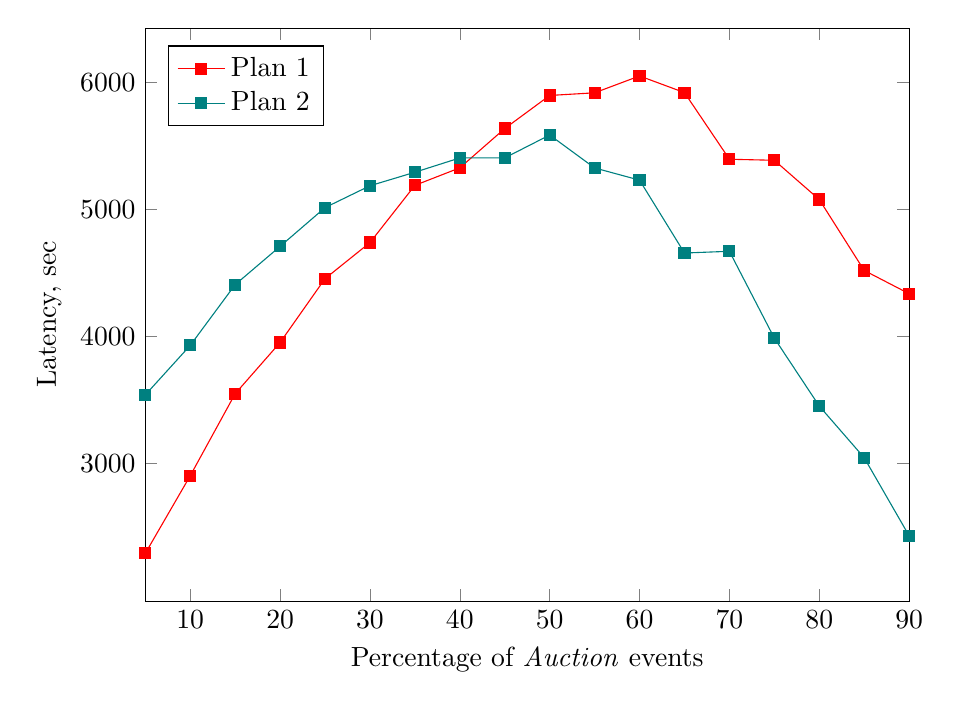
\begin{tikzpicture}
\begin{axis}[
    scale only axis=true,
    width=0.8\textwidth,
    height=0.6\textwidth,
    ytick={3000, 4000, 5000, 6000},
    yticklabels={3000, 4000, 5000, 6000},
    xmin=5, xmax=90,
    legend cell align=left,
    legend pos=north west,
    xlabel={Percentage of \textit{Auction} events},
    ylabel={Latency, sec},
    % x label style={at={(axis description cs:0.5,0.05)},anchor=north},
    % y label style={at={(axis description cs:0.125,0.5)},anchor=center},
]
\addplot[red,mark=square*,mark options={scale=1,solid}] coordinates {
    (5, 2294.73)
    (10, 2905.51)
    (15, 3550.93)
    (20, 3953.99)
    (25, 4456.47)
    (30, 4740.31)
    (35, 5190.68)
    (40, 5328.49)
    (45, 5637.89)
    (50, 5898.18)
    (55, 5918.89)
    (60, 6051.56)
    (65, 5920.56)
    (70, 5396.14)
    (75, 5387.98)
    (80, 5079.04)
    (85, 4520.84)
    (90, 4338.02)
};
\addplot[teal,mark=square*,mark options={scale=1,solid}] coordinates {
    (5, 3541.78)
    (10, 3931.32)
    (15, 4409.38)
    (20, 4710.69)
    (25, 5015.49)
    (30, 5187.45)
    (35, 5293.89)
    (40, 5406.6)
    (45, 5406.6)
    (50, 5586.84)
    (55, 5327.64)
    (60, 5231.65)
    (65, 4658.23)
    (70, 4671.75)
    (75, 3988.29)
    (80, 3453.75)
    (85, 3047.15)
    (90, 2432.85)
};
\legend{
    Plan 1\\
    Plan 2\\
}
\end{axis}
\end{tikzpicture}
            \captionsetup{justification=justified}
            \caption{Latency}
            \label{fig:latency_ratio}
    \end{subfigure}
    \hspace{5mm}
    \begin{subfigure}[b]{0.45\textwidth}
            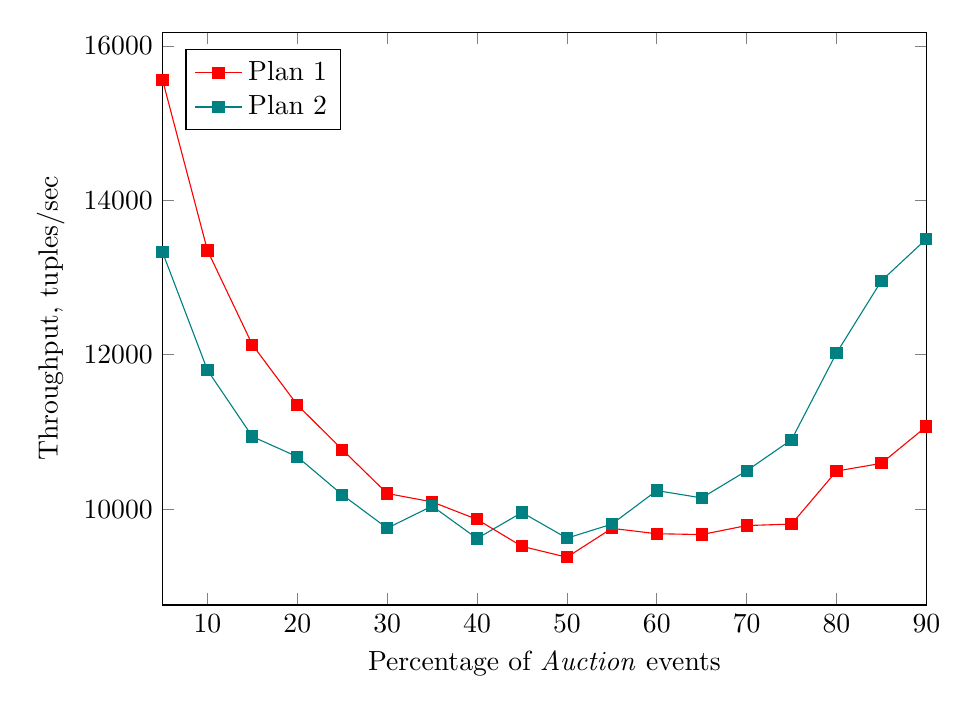
\begin{tikzpicture}
\begin{axis}[
    scale only axis=true,
    width=0.8\textwidth,
    height=0.6\textwidth,
    ytick={10000, 12000, 14000, 16000},
    % yticklabels={3000, 4000, 5000, 6000},
    xmin=5, xmax=90,
    legend cell align=left,
    legend pos=north west,
    xlabel={Percentage of \textit{Auction} events},
    ylabel={Throughput, tuples/sec},
    scaled ticks=false,
     /pgf/number format/.cd,
        use comma,
        1000 sep={}
    % x label style={at={(axis description cs:0.5,0.05)},anchor=north},
    % y label style={at={(axis description cs:0.125,0.5)},anchor=center},
]
\addplot[red,mark=square*,mark options={scale=1,solid}] coordinates {
    (5, 15559.14)
    (10, 13350.6)
    (15, 12128.8)
    (20, 11350.53)
    (25, 10771.7)
    (30, 10203.63)
    (35, 10094.87)
    (40, 9868.2)
    (45, 9519.33)
    (50, 9378.13)
    (55, 9752.17)
    (60, 9682.7)
    (65, 9671.77)
    (70, 9788.26)
    (75, 9807.67)
    (80, 10493.63)
    (85, 10594.13)
    (90, 11070.23)
};
\addplot[teal,mark=square*,mark options={scale=1,solid}] coordinates {
    (5,  13327.4)
    (10, 11800.3)
    (15, 10940.43)
    (20, 10679.2)
    (25, 10187.03)
    (30, 9754.23)
    (35, 10040.93)
    (40, 9621.1)
    (45, 9957.7)
    (50, 9625.23)
    (55, 9806.83)
    (60, 10241.43)
    (65, 10146.33)
    (70, 10497.6)
    (75, 10899.6)
    (80, 12021.9)
    (85, 12957.1)
    (90, 13499.33)
};
\legend{
    Plan 1\\
    Plan 2\\
}
\end{axis}
\end{tikzpicture}
            \captionsetup{justification=justified}
            \caption{Throughput}
            \label{fig:throughput_ratio}
    \end{subfigure}
    \caption{Latency and throughput for different ratios: out of 100 events, $|Person| = 5$, $|Auction|$ is the value on the $x$-axis, $|Bid| = 100 - |Person| - |Auction|$}
    \label{fig:ratio_plots}
\end{figure}

\begin{figure}[!ht]
    \centering
    \begin{subfigure}[b]{0.45\textwidth}
            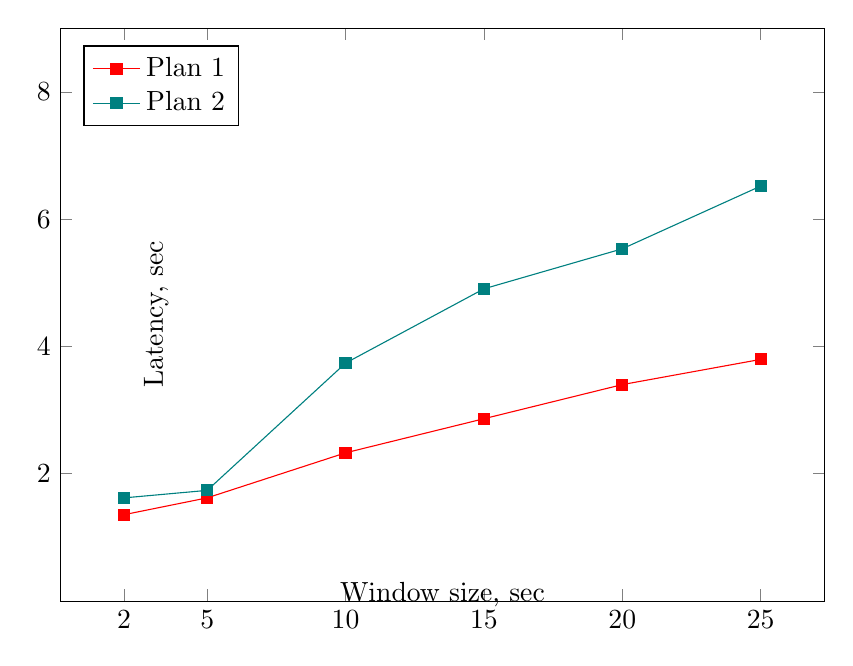
\begin{tikzpicture}
\begin{axis}[
    scale only axis=true,
    width=0.8\textwidth,
    height=0.6\textwidth,
    ymin = 0,
    ymax = 9000,
    ytick={2000, 4000, 6000, 8000},
    yticklabels={2, 4, 6, 8},
    xtick={2, 5, 10, 15, 20, 25},
    xticklabels={$2$, $5$, $10$, $15$, $20$, $25$},
    legend cell align=left,
    legend pos=north west,
    xlabel={Window size, sec},
    ylabel={Latency, sec},
    x label style={at={(axis description cs:0.5,0.05)},anchor=north},
    y label style={at={(axis description cs:0.125,0.5)},anchor=center},
]
\addplot[red,mark=square*,mark options={scale=1,solid}] coordinates {
(2,1357.67)
(5,1621.52)
(10,2328.99)
(15,2864.79)
(20,3400.97)
(25,3796.8)
};
\addplot[teal,mark=square*,mark options={scale=1,solid}] coordinates {
(2,1621.52)
(5,1739.10)
(10,3738.63)
(15,4905.88)
(20,5534.47)
(25,6519.64)
};
\legend{
    Plan 1\\
    Plan 2\\
}
\end{axis}
\end{tikzpicture}
            \captionsetup{justification=justified}
            \caption{$|Person|:|Auction|:|Bid|$ = 5:5:90}
            \label{fig:latency_window_5590}
    \end{subfigure}
    \hspace{1.25mm}
    \begin{subfigure}[b]{0.45\textwidth}
            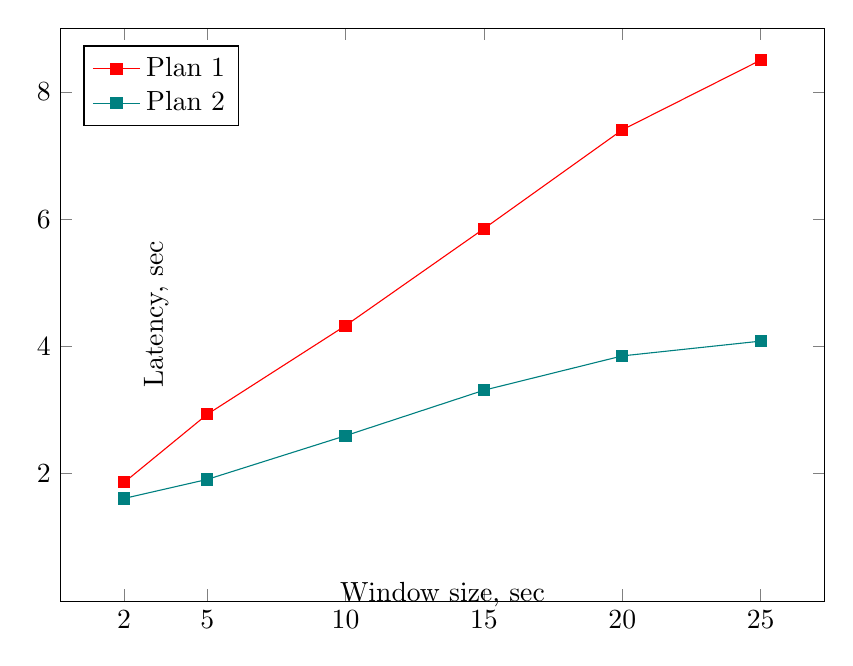
\begin{tikzpicture}
\begin{axis}[
    scale only axis=true,
    width=0.8\textwidth,
    height=0.6\textwidth,
    ymin = 0,
    ymax = 9000,
    ytick={2000, 4000, 6000, 8000},
    yticklabels={2, 4, 6, 8},
    xtick={2, 5, 10, 15, 20, 25},
    xticklabels={$2$, $5$, $10$, $15$, $20$, $25$},
    legend cell align=left,
    legend pos=north west,
    xlabel={Window size, sec},
    ylabel={Latency, sec},
    x label style={at={(axis description cs:0.5,0.05)},anchor=north},
    y label style={at={(axis description cs:0.125,0.5)},anchor=center},
]
\addplot[red, mark=square*, mark options={scale=1,solid}] coordinates {
(2,1864.23)
(5,2933.28)
(10,4327.74)
(15,5850.70)
(20,7403.71)
(25,8498.8)
};
\addplot[teal, mark=square*, mark options={scale=1,solid}] coordinates {
(2,1612.74)
(5,1911.15)
(10,2598.16)
(15,3312.47)
(20,3851.92)
(25,4083.96)
};
\legend{
    Plan 1\\
    Plan 2\\
}
\end{axis}
\end{tikzpicture}
            \captionsetup{justification=justified}
            \caption{$|Person|:|Auction|:|Bid|$ = 5:90:5}
            \label{fig:latency_window_5905}
    \end{subfigure}
    \caption{Latency for different window sizes and $|Person|:|Auction|:|Bid|$ ratios}
    \label{fig:latency_plots}
\end{figure}

\subsubsection{Latency}

We generated 1000000 events with the arrival rate of 10000 events per second and time-based windows of varying sizes.

Figure~\ref{fig:latency_ratio} 
demonstrates how latency changes depending on data characteristics. The $|Person|:|Auction|:|Bid|$ ratio impacts arrival rate for each kind of entities, thereby influencing latency. As expected, the plan in which \texttt{Person} and \texttt{Auction} are joined first delivers better results when the arrival rate of \texttt{Bid} records significantly overwhelms the rates of \texttt{Person} and \texttt{Auction} (the 5:5:90 ratio is an example of such a case), while the plan in which \texttt{Person} and \texttt{Bid} are joined first works best for cases where the rate of \texttt{Auction} records far exceeds those of \texttt{Person} and \texttt{Bid}. 

As Figures~\ref{fig:latency_window_5590} and~\ref{fig:latency_window_5905} demonstrate, the latency does not grow linearly as the window size increases. This is due to the fact that the join operator processes the records as they arrive instead of starting to process them only after the last record in the window has arrived, thus the results are ready to emerge shortly thereafter the arrival of the last record in the window.

Figure~\ref{fig:latency_diff_against_window_size} demonstrates how the difference in latency for the two execution plans changes with the window size. Since the difference grows as the window size increases, statistics-based optimization should provide an even bigger performance gain for larger windows.

\begin{figure}[!ht]
    \centering
    \begin{subfigure}[b]{0.45\textwidth}
            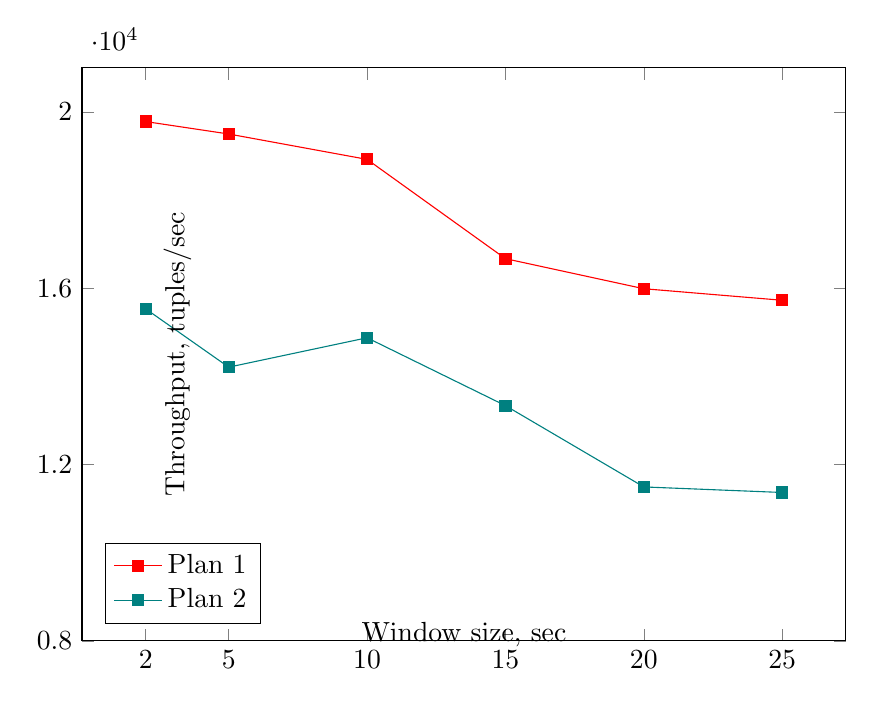
\begin{tikzpicture}
\begin{axis}[
    scale only axis=true,
    width=0.8\textwidth,
    height=0.6\textwidth,
    ymin = 8000,
    ymax = 21000,
    ytick={8000, 12000, 16000, 20000},
    %yticklabels={2, 4, 6, 8},
    xtick={2, 5, 10, 15, 20, 25},
    xticklabels={$2$, $5$, $10$, $15$, $20$, $25$},
    legend cell align=left,
    legend pos=south west,
    xlabel={Window size, sec},
    ylabel={Throughput, tuples/sec},
    x label style={at={(axis description cs:0.5,0.05)},anchor=north},
    y label style={at={(axis description cs:0.125,0.5)},anchor=center},
]
\addplot[red, mark=square*, mark options={scale=1,solid}] coordinates {
(2,19782.8)
(5,19500.8)
(10,18924.7)
(15,16671.4)
(20,15989.5)
(25,15727.7)
};
\addplot[teal, mark=square*, mark options={scale=1,solid}] coordinates {
(2,15532.8)
(5,14209.6)
(10,14876.5)
(15,13336.4)
(20,11491.7)
(25,11365.6)
};
\legend{
    Plan 1\\
    Plan 2\\
}
\end{axis}
\end{tikzpicture}
            \captionsetup{justification=justified}
            \caption{$|Person|:|Auction|:|Bid|$ = 5:5:90}
            \label{fig:throughput_window_5590}
    \end{subfigure}
    \hspace{1.25mm}
    \begin{subfigure}[b]{0.45\textwidth}
            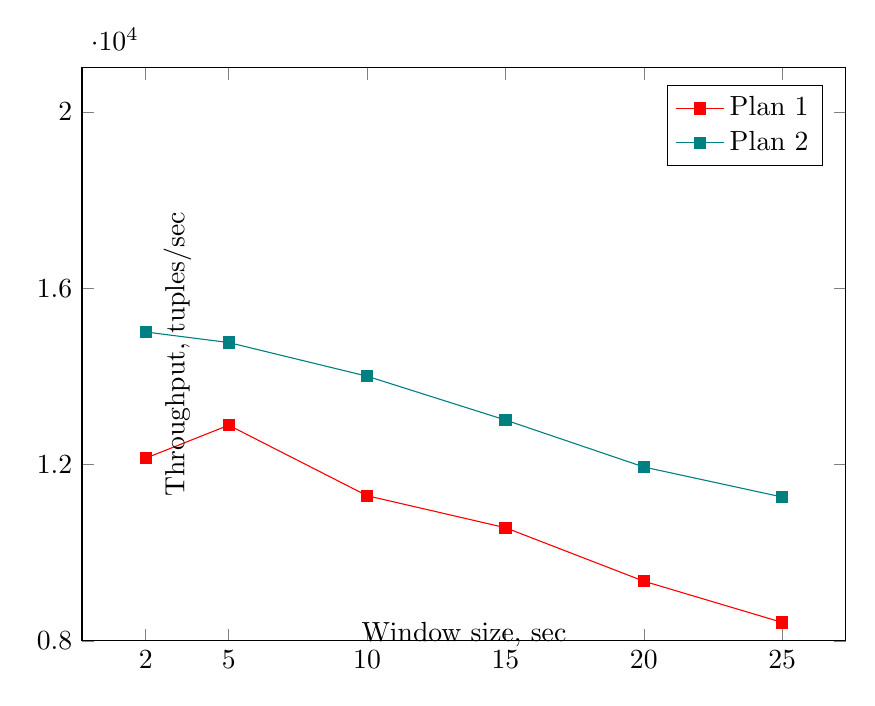
\begin{tikzpicture}
\begin{axis}[
    scale only axis=true,
    width=0.8\textwidth,
    height=0.6\textwidth,
    ymin = 8000,
    ymax = 21000,
    ytick={8000, 12000, 16000, 20000},
    %yticklabels={2, 4, 6, 8},
    xtick={2, 5, 10, 15, 20, 25},
    xticklabels={$2$, $5$, $10$, $15$, $20$, $25$},
    legend cell align=left,
    legend pos=north east,
    xlabel={Window size, sec},
    ylabel={Throughput, tuples/sec},
    x label style={at={(axis description cs:0.5,0.05)},anchor=north},
    y label style={at={(axis description cs:0.125,0.5)},anchor=center},
]
\addplot[red, mark=square*, mark options={scale=1,solid}] coordinates {
(2,12144.02)
(5,12892.16)
(10,11292.62)
(15,10566.26)
(20,9352.6)
(25,8416.64)
};
\addplot[teal, mark=square*, mark options={scale=1,solid}] coordinates {
(2,15007.76)
(5,14768.28)
(10,14004.28)
(15,13010.24)
(20,11943.94)
(25,11262.62)
};
\legend{
    Plan 1\\
    Plan 2\\
}
\end{axis}
\end{tikzpicture}
            \captionsetup{justification=justified}
            \caption{$|Person|:|Auction|:|Bid|$ = 5:90:5}
            \label{fig:throughput_window_5905}
    \end{subfigure}
    \caption{Throughput for different window sizes and $|Person|:|Auction|:|Bid|$ ratios}
    \label{fig:throughput_plots}
\end{figure}

\begin{figure}[!ht]
    \centering
    \begin{subfigure}[b]{0.45\textwidth}
            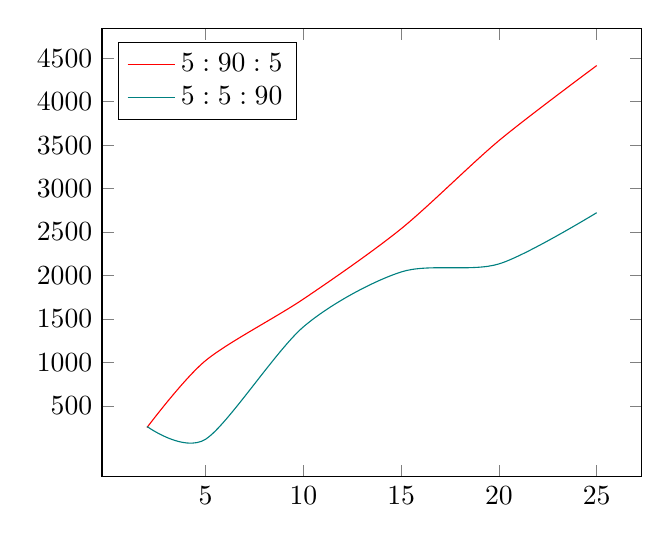
\begin{tikzpicture}
\begin{axis}[
    ytick={500, 1000, 1500, 2000, 2500, 3000, 3500, 4000, 4500},
    yticklabels={$500$, $1000$, $1500$, $2000$, $2500$, $3000$, $3500$, $4000$, $4500$},
    xtick={5, 10, 15, 20, 25},
    xticklabels={$5$, $10$, $15$, $20$, $25$},
    legend cell align=left,
    legend pos=north west
]
\addplot[smooth, red] coordinates {
(2,251.49)
(5,1022.13)
(10,1729.58)
(15,2538.23)
(20,3551.79)
(25,4414.84)
};
\addplot[smooth, teal] coordinates {
(2,263.85)
(5,117.58)
(10,1409.64)
(15,2041.09)
(20,2133.5)
(25,2722.84)
};
\legend{
    $5:90:5$\\
    $5:5:90$\\
}
\end{axis}
\end{tikzpicture}
            \captionsetup{justification=justified}
            \caption{Latency difference}
            \label{fig:latency_diff_against_window_size}
    \end{subfigure}
    \hspace{1.25mm}
    \begin{subfigure}[b]{0.45\textwidth}
        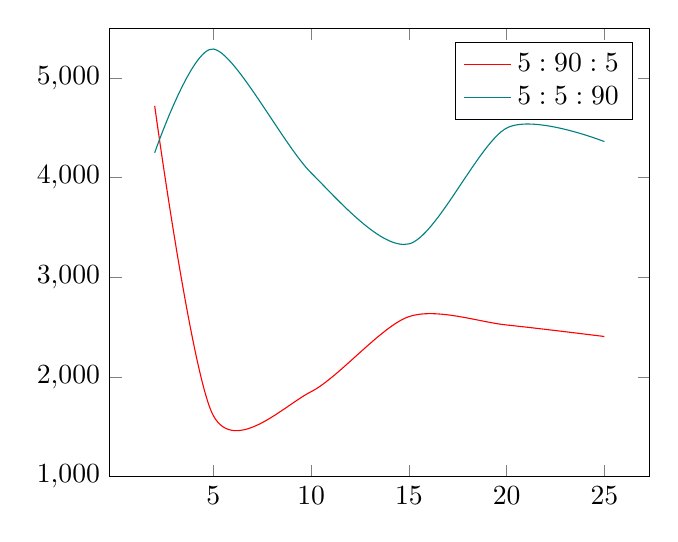
\begin{tikzpicture}
\begin{axis}[
    ymin=1000, ymax=5500,
    xtick={5, 10, 15, 20, 25},
    xticklabels={$5$, $10$, $15$, $20$, $25$},
    legend cell align=left,
    legend pos=north east
]
\addplot[smooth, red] coordinates {
(2,4721.1)
(5,1611.0)
(10,1851.7)
(15,2604.9)
(20,2521.2)
(25,2405.5)
};
\addplot[smooth, teal] coordinates {
(2,4250.0)
(5,5291.2)
(10,4048.2)
(15,3335)
(20,4497.8)
(25,4362.1)
};
\legend{
    $5:90:5$\\
    $5:5:90$\\
}
\end{axis}
\end{tikzpicture}
        \captionsetup{justification=justified}
        \caption{Throughput difference}
        \label{fig:throughput_diff_against_window_size}
    \end{subfigure}
    \caption{Difference in latency and throughput for Plans 1 and 2}
    \label{fig:latency_and_throughput_difference}
\end{figure}

\subsubsection{Throughput}

The parameters for throughput estimation were the same as for the latency estimation. As Figure \ref{fig:throughput_ratio} shows, Plan 2 delivers higher throughput in case of the arrival rate of \texttt{Auction} significantly exceeding that of \texttt{Person} and \texttt{Bid}, while Plan 2 performs better in case of the arrival rate of \texttt{Bid} being significantly higher. This corresponds with the latency measurements. Throughput decreases with the increase of window size, as shown in Figures \ref{fig:throughput_window_5590} and \ref{fig:throughput_window_5905}. Throughput difference remains constant and does not depend on the window size, Figure \ref{fig:throughput_diff_against_window_size} demonstrates.

% \begin{figure*}[t!]
%     \begin{subfigure}[b]{0.32\textwidth}
%             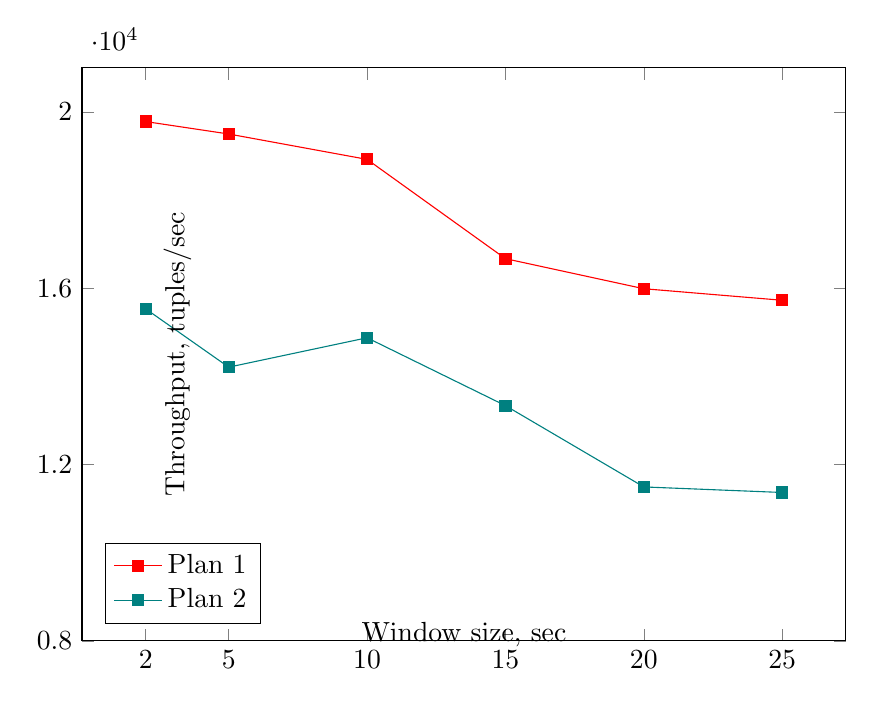
\begin{tikzpicture}
\begin{axis}[
    scale only axis=true,
    width=0.8\textwidth,
    height=0.6\textwidth,
    ymin = 8000,
    ymax = 21000,
    ytick={8000, 12000, 16000, 20000},
    %yticklabels={2, 4, 6, 8},
    xtick={2, 5, 10, 15, 20, 25},
    xticklabels={$2$, $5$, $10$, $15$, $20$, $25$},
    legend cell align=left,
    legend pos=south west,
    xlabel={Window size, sec},
    ylabel={Throughput, tuples/sec},
    x label style={at={(axis description cs:0.5,0.05)},anchor=north},
    y label style={at={(axis description cs:0.125,0.5)},anchor=center},
]
\addplot[red, mark=square*, mark options={scale=1,solid}] coordinates {
(2,19782.8)
(5,19500.8)
(10,18924.7)
(15,16671.4)
(20,15989.5)
(25,15727.7)
};
\addplot[teal, mark=square*, mark options={scale=1,solid}] coordinates {
(2,15532.8)
(5,14209.6)
(10,14876.5)
(15,13336.4)
(20,11491.7)
(25,11365.6)
};
\legend{
    Plan 1\\
    Plan 2\\
}
\end{axis}
\end{tikzpicture}
%             \captionsetup{justification=justified}
%             \caption{$|Person|:|Auction|:|Bid|$ = 5:5:90}
%             \label{fig:throughput_window_5590}
%     \end{subfigure}
%     \hspace{2mm}
%     \begin{subfigure}[b]{0.32\textwidth}
%             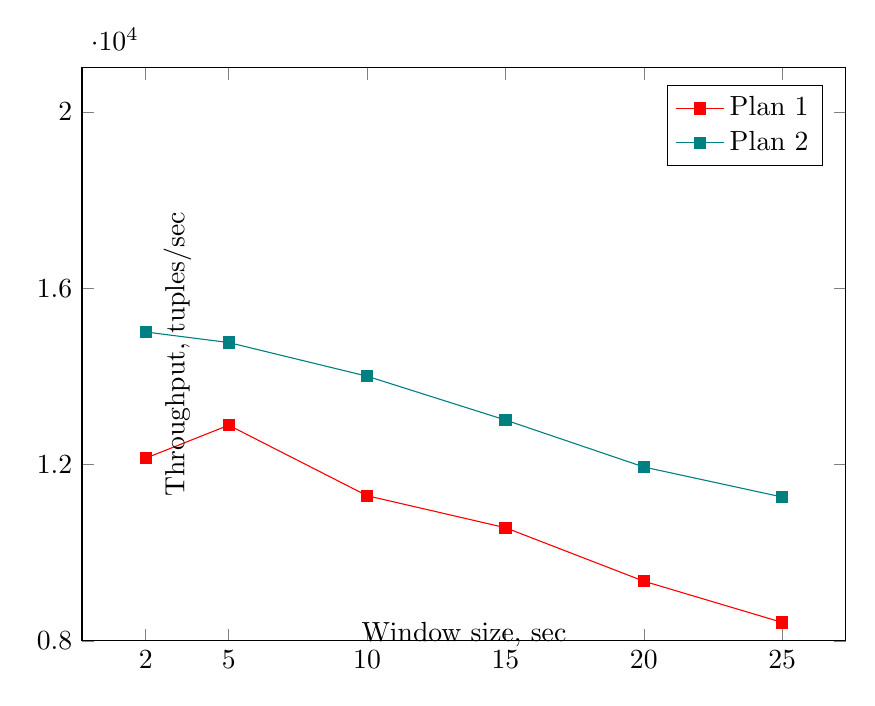
\begin{tikzpicture}
\begin{axis}[
    scale only axis=true,
    width=0.8\textwidth,
    height=0.6\textwidth,
    ymin = 8000,
    ymax = 21000,
    ytick={8000, 12000, 16000, 20000},
    %yticklabels={2, 4, 6, 8},
    xtick={2, 5, 10, 15, 20, 25},
    xticklabels={$2$, $5$, $10$, $15$, $20$, $25$},
    legend cell align=left,
    legend pos=north east,
    xlabel={Window size, sec},
    ylabel={Throughput, tuples/sec},
    x label style={at={(axis description cs:0.5,0.05)},anchor=north},
    y label style={at={(axis description cs:0.125,0.5)},anchor=center},
]
\addplot[red, mark=square*, mark options={scale=1,solid}] coordinates {
(2,12144.02)
(5,12892.16)
(10,11292.62)
(15,10566.26)
(20,9352.6)
(25,8416.64)
};
\addplot[teal, mark=square*, mark options={scale=1,solid}] coordinates {
(2,15007.76)
(5,14768.28)
(10,14004.28)
(15,13010.24)
(20,11943.94)
(25,11262.62)
};
\legend{
    Plan 1\\
    Plan 2\\
}
\end{axis}
\end{tikzpicture}
%             \captionsetup{justification=justified}
%             \caption{$|Person|:|Auction|:|Bid|$ = 5:90:5}
%             \label{fig:throughput_window_5905}
%     \end{subfigure}
%     \hspace{2mm}
%     \begin{subfigure}[b]{0.32\textwidth}
%             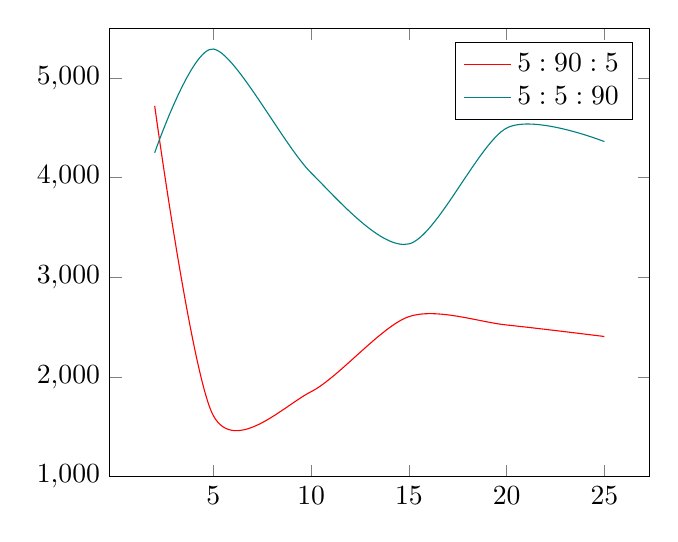
\begin{tikzpicture}
\begin{axis}[
    ymin=1000, ymax=5500,
    xtick={5, 10, 15, 20, 25},
    xticklabels={$5$, $10$, $15$, $20$, $25$},
    legend cell align=left,
    legend pos=north east
]
\addplot[smooth, red] coordinates {
(2,4721.1)
(5,1611.0)
(10,1851.7)
(15,2604.9)
(20,2521.2)
(25,2405.5)
};
\addplot[smooth, teal] coordinates {
(2,4250.0)
(5,5291.2)
(10,4048.2)
(15,3335)
(20,4497.8)
(25,4362.1)
};
\legend{
    $5:90:5$\\
    $5:5:90$\\
}
\end{axis}
\end{tikzpicture}
%             \captionsetup{justification=justified}
%             \caption{Throughput difference for Plans 1 and 2}
%             \label{fig:throughput_diff_against_window_size}
%     \end{subfigure}
%     \caption{Throughput for different window sizes and $|Person|:|Auction|:|Bid|$ ratios}
%     \label{fig:throughput_plots}
% \end{figure*}


\subsection{Discussion}

The results of our experiments demonstrate that streaming query execution performance depends on the plan used for the execution, and the optimality of the plan depends on the data characteristics, which proves the necessity of adaptive optimization of streaming queries. Particularly, the first steps towards adaptive optimization should be predicting statistics for each window and performing runtime graph migration, since the results of the experiments show that even the current planners, such as the Volcano query planner \cite{graefe1993volcano} used in Apache Calcite, which are unaware of whether the data comes from a stream or a table, could use those statistics to produce a better execution plan. These two challenges will be the focus of our future work. After that, the planner can be enhanced by introducing distributed streaming systems-specific operators and their costs.




\section{Related work}
\label {sec:fs-optimization-related-work}

We structure the related work into three areas: database query optimization, optimization of streaming queries, and predicting data statistics for queries using machine learning techniques.

Early efforts in database query optimization include the System R optimizer \cite{selinger1979access}, which introduced a dynamic programming algorithm for finding an optimal execution plan; the Starburst optimizer \cite{haas1989extensible}, which proposed new rule-based optimization techniques; and others: a survey chapter on query optimization in relational databases can be found in \cite{Neumann2018optimization}. Our particular interest lies in the areas of query optimization in distributed database systems and adaptive query optimization. The former has been described in \cite{kossmann2000thestate}; a detailed survey \cite{deshpande2007adaptive} is a good reference for the latter. Adaptive optimization of streaming SQL queries is different from database optimization: while in databases the execution plan is modified during the execution of a query, in streaming systems the plan should be changed after a window has been processed but before the next window processing has started; moreover, database data is static during the query execution while streaming data is continuously updated.

An overview of streaming query optimizations can be found in \cite{hirzel2014catalog}: most of these optimizations can be classified as rule-based and are applied statically at compilation time, although dynamic versions are listed for several of these; we are interested in adaptive optimization at runtime. Various works explore adaptive optimization of streaming queries: \cite{babu2004adaptive} focuses on finding the optimal order of pipelined filter operators, with possible reordering at runtime; it uses the current known data statistics while we are interested in predicting the next window statistics and using those. Other works focus on physical level adaptive optimizations: one such study can be found in \cite{grulich2020grizzly}; we are interested in logical level optimization instead. Another approach for physical optimization is discussed in~\cite{kroll2019arc}. It is based on the intermediate representation (IR) of the streaming queries, which supports a wide range of physical optimizations: operator redundancy elimination, operator separation, and fusion~\cite{hirzel2014catalog}. However, the optimizations based on operator reordering is limited within this method due to the lack of algebraic properties that is usually built around the relational model.

Previous works on execution graph reconfiguration in runtime, including Eddies project~\cite{10.1145/335191.335420} and StreaMon~\cite{10.1145/1007568.1007702}, primarily study centralized stream processing, but, as we mentioned in Section~\ref{sec:fs-optimization-challenges}, many issues origin from the distributed environment. The approach for state migration in distributed environment introduced in~\cite{10.14778/3329772.3329777} can be applied as a building block for the general graph reconfiguration mechanism.

Some studies (\cite{krishnan2018learning, marcus2019neo}) use machine learning to predict optimal execution plans, while others explore join cardinality prediction. Database cardinality prediction techniques can be categorized as either query-driven or data-driven. Query-driven prediction models learn on sets of queries; among studies employing this approach are \cite{liu2015cardinality, CHEN20211047, kipf2018learned, ortiz2019empirical}, which use neural networks. Data-driven prediction models, described in \cite{hilprecht2020deepdb} and \cite{yang2020neurocard}, are trained on data without queries and attempt to learn characteristics such as distribution of single attributes as well as joint distributions of multiple attributes. Neither of these approaches fit the streaming queries scenario: SPEs are executing the same query on each subsequent window, rendering query-driven approaches unusable, and the data is continuously updating, which means data-driven approaches are not employable either. Additionally, neural networks might not be the best choice of a learning model for a small amount of data contained in a single window; instead, it would potentially be more beneficial to use a model similar to \cite{street2001ensemble}, a fixed-size ensemble of heuristically replaced classifiers. Predicting statistics for streaming queries might yield better results than for database queries since the query is being run on different subsequent windows for an extended period of time, unlike in databases, where each new query is run separately from its predecessors. This could be advantageous in predicting statistics not only for the next input window but for intermediate execution results as well.

% cost-based database optimization

% physical-level/non-specific to sql database optimizations

% predicting cardinality using ML in databases or in streams even if that exists

% in-flight graph migration, possibly included in sections about optimizations above

% TODO move this into the machine learning section

% On the topic of predicting data statistics, it must be noted that while there have been various attempts at predicting cardinality in databases (\cite{liu2015cardinality, kipf2018learned, ortiz2019empirical, CHEN20211047}), predicting statistics for streaming queries might yield better results since the query is being run on different subsequent windows for an extended period of time, unlike in databases, where each new query is run separately from its predecessors. This could be advantageous in predicting statistics not only for the next window but for intermediate execution results as well.


% The
% methods presented in this paper take advantage of plentiful
% data, building separate classifiers on sequential chunks of

% training points. These classifiers are combined into a fixed-
% size ensemble using a heuristic replacement strategy.

%rate-based optimization of streaming queries добавить

\section{Conclusion}
\label {sec:fs-optimization-conclusion}
In this paper, we introduced  the concept  of adaptive optimization of streaming SQL queries in distributed stream processing engines and highlighted the differences between adaptive optimization 	for database and stream queries. 
We argued the necessity of adaptive query optimization at both  logical and the physical levels.
We identify the following challenges in realization of  optimization techniques for streaming queries: 
fetching and predicting data statistics, 
using predicted statistics for the query optimization, and migrating the execution graph in runtime once the statistics have changed enough that the previous execution plan becomes suboptimal. 

We presented a running example of a streaming SQL query and performed experiments on this query and its different possible execution graphs to demonstrate the possibility of a gain in performance should the graph be adapted to the data statistics. 

\bibliographystyle{splncs04}
\bibliography{bibliography/flame-stream}

\end{document}

\endinput
